\chapter{SysML v2}
\section{Bevezetés}
A SysML második verzióját az első verzió használata során tanultak alapjára építették, de azt teljesen átdolgozták.
Ígéretei szerint növeli az modell alapú rendszertervezés adaptációját és hatékonyságát.
Ehhez az új változat (többek között):
\begin{itemize}
    \item növeli a nyelv pontosságát és kifejezőképességét.
    \item fokozza a konzisztenciát és integrációt más nyelvekkel
    \item növeli az átjárhatóságot más mérnöki modellekkel és eszközökkel
\end{itemize}

Az új nyelv két részből áll: 1, maga a SysML v2 nyelv és 2, SysML v2 API \& Services.
Az előbbit 2017 decemberében terjesztették elő RFP formájában, míg az utóbbira 2018 júniusában került sor.
A végleges specifikáció 2022 4. negyedévében várható, bár ez még jóváhagyásra vár.

\section{Nyelvi újdonságok}
A nyelv belülről teljesen megváltozott, az UML-től való függőséget megszüntették es egy új metamodell alapján fejlesztették.
A nyelv felépítése a \ref{fig:v2meta}. ábrán látható. Mint az látható, a SysML nyelv a KerML nyelvre épül rá.

A KerML metamodellje biztosítja a különböző domain specifikus verziók közti átjárhatóságot.

\begin{figure}
    \centering
    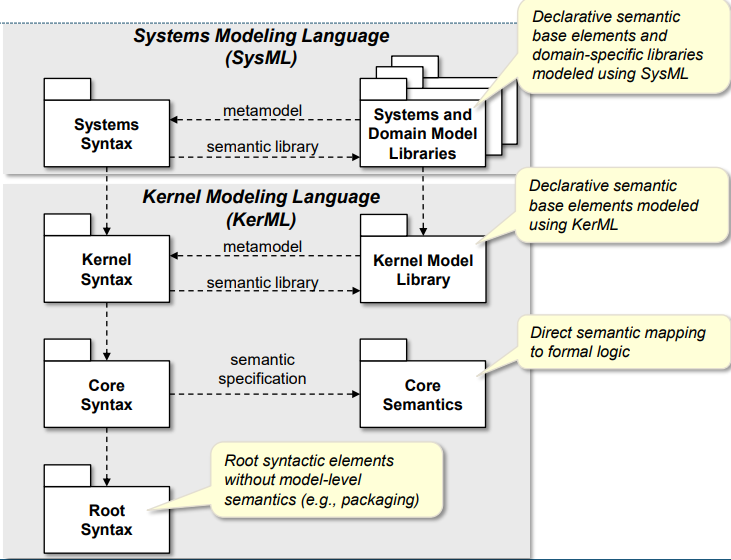
\includegraphics[width=150mm, keepaspectratio]{figures/v2_metamodel.png}
    \caption{A SysML v2 nyelv felépítése. Forrás: SysML v2 Update, 2021}
    \label{fig:v2meta}
\end{figure}

A SysML v2 nyelvhez készítettek egy szöveges szintaxist is a jobban támogatható automatizálhatósághoz, mely a grafikus változattal egyenértékű.
A nyelv képességeit a \ref{fig:v2_mapping} ábra mutatja.

\begin{figure}
    \centering
    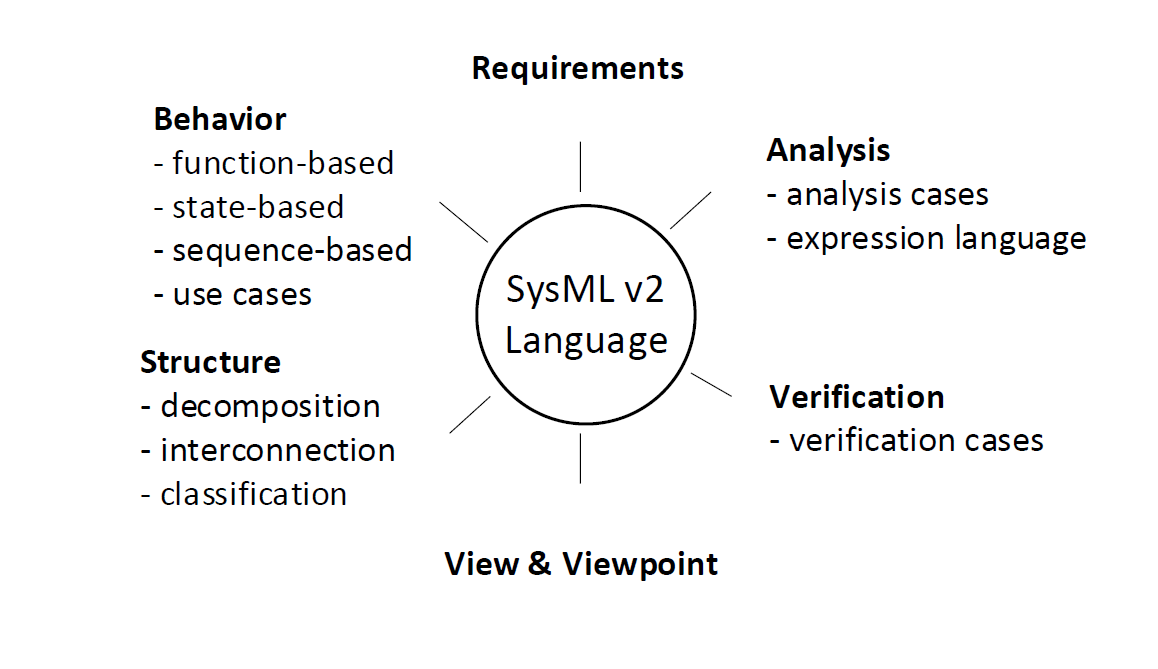
\includegraphics[width=100mm, keepaspectratio]{figures/v2_capabilities.png}
    \caption{SysML v2 képességei. Forrás: Intro to the SysML v2 Language-Graphical Notation}
    \label{fig:v2_mapping}
\end{figure}